\section{Les 4 -- nevenklassen, quotiëntgroepen}

\begin{barbox}[red][red!10]
    \emoji{warning} volgens de prof moet sectie 3.2 uit hoofdstuk 3 niet gekend zijn, maar dit was de helft van les 4 dus ik heb het opgenomen in deze samenvatting.
\end{barbox}

\textbf{\underbar{herinner:}} Een groep $\langle G,\ * \rangle$ is een verzameling met een samenstellingswet (bewerking) die een afbeelding $G \times G \to G: (g,\ h) \mapsto g*h$ is die voldoet aan:
\begin{enumerate}
    \item Overal bepaald (zit in definitie \emph{afbeelding} (\Cref{def:h2_afbeelding}))
    \item Associativiteit
    \item Er bestaat een neutraal element
    \item Symmetriseerbaar: $\forall g \in G : \exists g^{-1}$
\end{enumerate}

\begin{nicedefinition}*[Homomorfisme]
    \nextpart[]*
    Een \textcolor{PineGreen!75!black}{\textbf{homomorfisme}} tussen groepen $\langle G,\ * \rangle$ en $\langle H,\ \triangleright \rangle$ is een afbeelding $\varphi : G \to H$ die compatibel is met die groepswetten. Maw. die voldoet aan:
    \begin{equation*}
        \varphi(x * y) = \varphi(x) \triangleright \varphi(y) \qquad \forall x,y \in G
    \end{equation*} 

    \vspace{0.25cm}

    Een \textcolor{PineGreen!75!black}{\textbf{isomorfisme}} is een bijectief homomorfisme.
\end{nicedefinition}

\textbf{\underline{Notatie:}} Als er een isomorfisme $\varphi : G \to H$ bestaat, dan schrijf je $G \cong H$.

\begin{niceexercise}
    Zij $\varphi : G \to H$ een homomorfisme. Dan geldt:
    \begin{enumerate}
        \item Het neutraal element wordt altijd op het neutraal element afgebeeld: $\varphi(e_G) = e_H$
        \item $\varphi(g^{-1}) = \varphi(g)^{-1} \quad \forall g \in G$
        \item Als $\varphi$ een isomorfisme is, dan is $\varphi^{-1}$ het ook.
    \end{enumerate}
\end{niceexercise}
\textbf{\underline{Oplossing:}}


\textbf{1.} We tonen aan dat
\begin{equation*}
    \varphi(e_G) = e_H
\end{equation*}
Omdat $e_G$ het neutraal element is in $G$, geldt:
\begin{equation*}
    e_G * e_G = e_G
\end{equation*}
Pas dan $\varphi$ toe op beide kanten:
\begin{equation*}
    \varphi(e_G * e_G) = \varphi(e_G)
\end{equation*}

Omdat $\varphi$ een homomorfisme is, geldt:
\begin{equation*}
    \varphi(e_G * e_G) = \varphi(e_G) \triangleright \varphi(e_G)
\end{equation*}
Dus:
\begin{equation*}
    \varphi(e_G) \triangleright \varphi(e_G) = \varphi(e_G)
\end{equation*}
vermenigvuldig nu links met $\varphi(e_G)^{-1}$ in $H$:
\begin{equation*}
    \varphi(e_G)^{-1} \triangleright \bigl(\ \varphi(e_G) \triangleright \varphi(e_G) \ \bigr) = \underbrace{\varphi(e_G)^{-1} \triangleright \varphi(e_G)}_{e_H}
\end{equation*}
Door associativiteit krijgen we:
\begin{equation*}
    \bigl(\ \varphi(e_G)^{-1} \triangleright \varphi(e_G)\ \bigr) \triangleright \varphi(e_G) = e_H
\end{equation*}
Dus:
\begin{equation*}
    e_H \triangleright \varphi(e_G) = e_H
\end{equation*}
en omdat $e_H$ het neutraal element van $H$ is:
\begin{equationbox}*[Goldenrod][Goldenrod!10]
    \varphi(e_G) = e_H
\end{equationbox}

\hrule
\textbf{2.} We tonen aan dat
\begin{equation*}
    \varphi(g^{-1}) = \varphi(g)^{-1}
\end{equation*}
Neem $g \in G$. Dan geldt:
\begin{equation*}
    g * g^{-1} = e_G
\end{equation*}
Pas $\varphi$ toe:
\begin{equation*}
    \varphi(g * g^{-1}) = \varphi(e_G)
\end{equation*}
Omdat $\varphi$ een homomorfisme is:
\begin{equation*}
    \varphi(g) \triangleright \varphi(g^{-1}) = \varphi(e_G)
\end{equation*}
Uit (1) weten we dat $\varphi(e_G) = e_H$. Dus:
\begin{equation*}
    \varphi(g) \triangleright \varphi(g^{-1}) = e_H
\end{equation*}
Dit betekent dat $\varphi(g^{-1})$ een rechter-inverse is van $\varphi(g)$. In een groep is de inverse uniek, dus:
\begin{equationbox}*[Goldenrod][Goldenrod!10]
    \varphi(g^{-1}) = \varphi(g)^{-1}
\end{equationbox}

\hrule
\textbf{3.} Stel nu dat $\varphi$ een isomorfisme is. Dan is $\varphi$ bijectief, dus bestaat de inverse afbeelding
\begin{equation*}
    \varphi^{-1} : H \to G
\end{equation*}
We moeten dus aantonen dat $\varphi^{-1}$ ook een homomorfisme is. Neem willekeurige elementen $x,y \in H$. Omdat $\varphi$ surjectief is, bestaan er $a,b \in G$ zodat:
\begin{equation*}
    x = \varphi(a) \qquad \text{en} \qquad y = \varphi(b)
\end{equation*}
Dan geldt:
\begin{equation*}
    x \triangleright y = \varphi(a) \triangleright \varphi(b)
\end{equation*}
Omdat $\varphi$ een homomorfisme is:
\begin{equation*}
    \varphi(a) \triangleright \varphi(b) = \varphi(a*b)
\end{equation*}
Dus:
\begin{equation*}
    x \triangleright y = \varphi(a * b)
\end{equation*}
Pas nu $\varphi^{-1}$ toe:
\begin{equation*}
    \varphi^{-1}(x \triangleright y) = \varphi^{-1}(\varphi(a * b))
\end{equation*}
Omdat $\varphi^{-1}$ de inverse afbeelding is van $\varphi$, krijg je:
\begin{equation*}
    \varphi^{-1}(x \triangleright y) = a * b
\end{equation*}
Maar omdat $x = \varphi(a)$ en $y = \varphi(b)$, geldt:
\begin{equation*}
    a = \varphi^{-1}(x) \qquad \text{en} \qquad b = \varphi^{-1}(y)
\end{equation*}
Dus:
\begin{equation*}
    \varphi^{-1}(x \triangleright y) = \varphi^{-1}(x) * \varphi^{-1}(y)
\end{equation*}
Dit geldt voor alle $x,y\in H$, dus $\varphi^{-1}$ is een homomorfisme. Omdat $\varphi^{-1}$ bovendien bijectief is, is $\varphi^{-1}$ een isomorfisme.

\textbf{\underbar{Voorbeelden:}}
\begin{itemize}
    \item Verdubbelingsafbeelding op de gehele getallen: $\langle \mathbb{Z}, + \rangle \to \langle \mathbb{Z},+ \rangle : x \mapsto 2x$ is een homomorfisme.
    \item $\langle \mathbb{R},+ \rangle \to \langle \mathbb{R}_{>0},\cdot \rangle : x \mapsto e^x$ is een isomorfisme. Want: definieer:
    \begin{equation*}
        \varphi : \mathbb{R} \to \mathbb{R}_{>0} : x \mapsto e^x
    \end{equation*}
    We tonen eerst aan dat $\varphi$ een homomorfisme is. Neem $x,y \in \mathbb{R}$. Dan geldt:
    \begin{equation*}
        \varphi(x+y) = e^{x+y}
    \end{equation*}
    Omdat
    \begin{equation*}
        e^{x+y} = e^x \cdot e^y,
    \end{equation*}
    krijg je:
    \begin{equation*}
        \varphi(x+y) = e^x \cdot e^y.
    \end{equation*}

    Dus:
    \begin{equation*}
        \varphi(x+y) = \varphi(x) \cdot \varphi(y)
    \end{equation*}

    Daarom is $\varphi$ een homomorfisme van $\langle \mathbb{R},+ \rangle$ naar $\langle \mathbb{R}_{>0},\cdot \rangle$.

    We tonen nu aan dat $\varphi$ een bijectief is. De inverse afbeelding is
    \begin{equation*}
        \varphi^{-1} : \mathbb{R}_{>0} \to \mathbb{R} : y \mapsto ln(y)
    \end{equation*}
    Inderdaad:
    \begin{equation*}
        \varphi^{-1}(\varphi(x)) = \ln(e^x) = x \qquad \forall x \in \mathbb{R},
    \end{equation*}
    en
    \begin{equation*}
        \varphi(\varphi^{-1}(y)) = e^{\ln(y)} = y \qquad \forall y \in \mathbb{R}_{>0}.
    \end{equation*}
    Dus $\varphi$ is bijectief. Aangezien $\varphi$ een bijectief homomorfisme is, is $\varphi$ een isomorfisme.

    \item $GL_n(\mathbb{R}) = \langle\{M \in \mathbb{R}^{n \times n} \mid det(M) \neq 0\}, \cdot \rangle \to \langle \mathbb{R}\backslash\{0\},\cdot \rangle : M \mapsto det(M)$ is een homomorfisme. Denk aan $det(AB) = det(A)det(B)$. Deze groep noemt de \inlinetext{General Linear Group}.
    
    \item $\langle \mathbb{Z}_4,+ \rangle \to \mathbb{Z}_5\backslash\{\bar{0}\},\cdot : \begin{cases}
        \bar{0} \mapsto \bar{1} \\
        \bar{1} \mapsto \bar{2}
    \end{cases}$ is een isomorfisme, want $\mathbb{Z}_4$ is cyclisch en wordt voortgebracht door $\bar{1}$ (zie later). Daardoor ligt de rest van de afbeelding vast. Namelijk:
    \begin{equation*}
        \bar{2} = \bar{1} + \bar{1}
    \end{equation*}
    dus:
    \begin{equation*}
        \varphi(\bar{2}) = \varphi(\bar{1} + \bar{1}) = \bar{1} \cdot \bar{1} = \bar{2} \cdot \bar{2} = \bar{4}
    \end{equation*}
    En:
    \begin{equation*}
        \bar{3} = \bar{1} + \bar{1} + \bar{1}
    \end{equation*}
    dus:
    \begin{equation*}
        \varphi(\bar{3}) = \bar{2}^3 = \bar{8} = \bar{3}
    \end{equation*}
\end{itemize}

\begin{nicetheorem}*[Deelgroep]\label{theo:H3_deelgroep}
    \nextpart[]*
    Zij $\langle G,* \rangle$ een groep. Zij $H \subset G$ een deelverzameling en $H \neq \emptyset$. Dan is $\langle H,* \rangle$ ook een groep. Meer specifiek een \textcolor{red!75!black}{\textbf{deelgroep}} van $G$ \emph{asa}
    \begin{itemize}
        \item $H*H \subseteq H$, dwz. $a,b \in H \implies a*b \in H$. Dan kan je "$*$" zien als een bewerking op $H$. $H$ is stabiel voor de bewerking "$*$".
        \item $H^{-1} \subseteq H$, dwz. als $a \in H \implies a^{-1} \in H$.
    \end{itemize}
\end{nicetheorem}

\textbf{\underbar{Voorbeelden:}}
\begin{itemize}
    \item $\langle \mathbb{R}_{>},\cdot \rangle$ is een deelgroep van $\langle \mathbb{R}\backslash\{0\},\cdot \rangle$
    \item De veelvouden van $m$: $\langle \mathbb{Z},+\rangle$ is een deelgroep van $\langle\mathbb{Z},+\rangle$, $\forall m \ge 1$
    \item $\langle SL_n(\mathbb{R}) = \{ M \in \mathbb{R}^{n \times n} \mid det(M)=1 \} \rangle$ is een deelgroep van alle matrices $\{A \in \mathbb{R}^{n \times n} \mid det(A) \neq 0\} = GLn(\mathbb{R})$. $SL_n(\mathbb{R})$ noemt men de \inlinetext{Special Linear group}.
    \item $\langle A_n = \{\sigma \in S_n \mid \text{sign}(\sigma)=+1\}, \circ \rangle$ is een deelgroep van $S_n$. $A_n$ noemt men de \newline\inlinetext{Alternating group}. Dus een deelgroep met enkel \textbf{even permutaties}.
\end{itemize}

\begin{nicetheorem}*[Stelling van Cayley]
    Zij $\langle G,* \rangle$ een groep. Dan is $G$ isomorf met een deelgroep van $\langle S(G) = \{\text{bijecties } G \to G\},\circ \rangle$. 
    
    \vspace{0.25cm}
    
    $\langle S(G),\circ \rangle$ is de \inlinetext{symmetrische groep} op $G$, dit is de verzameling van alle permutaties op $G$, dwz. alle bijecties van $G$ naar zichzelf.
    \nextpart[Bewijs.]*
    Stel elk groepselement $g$ voor als een permutatie van $G$. Dus $\forall g \in G$ definiëren we:
    \begin{equation*}
        \pi_g : G \to G : x \mapsto g*x = \pi_g(x)
    \end{equation*}
    Dit is de afbeelding die elk element $x \in G$ links vermenigvuldigt met $g$.

    Defininieer nu
    \begin{eqnarray}
        X = \{\pi_g \mid g \in G\}
    \end{eqnarray}

    We willen nu aantonen dat $X$ een deelgroep is van $S(G)$ en dat
    \begin{equation*}
        G \cong X
    \end{equation*}

    \vspace{0.25cm}

    \textbf{1) We tonen eerst aan dat $\pi_g$ een bijectie is.} Neem $g \in G$. We zoeken een inverse afbeelding voor $\pi_g$ en beweren dat
    \begin{equation*}
        \pi_g^{-1} = \pi_{g^{-1}}
    \end{equation*} 
    Inderdaad, neem $x \in G$, dan geldt:
    \begin{equation*}
        (\pi_{g^{-1}} \circ \pi_g)(x) = \pi_{g^{-1}}(\pi_g(x))
    \end{equation*}
    Omdat $\pi_g(x) = g*x$, krijg je:
    \begin{equation*}
        \pi_{g^{-1}}(\pi_g(x)) = \pi_{g^{-1}}(g*x)
    \end{equation*}
    Per definitie van $\pi_{g^{-1}}$:
    \begin{equation*}
        \pi_{g^{-1}}(g*x) = g^{-1}(g*x)
    \end{equation*}
    Door associativiteit:
    \begin{equation*}
        g^{-1}*(g*x) = (g^{-1}*g)*x
    \end{equation*}
    Omdat $g^{-1}*g = e$, volgt:
    \begin{equation*}
        (g^{-1}*g)*x = e*x = x
    \end{equation*}
    Dus:
    \begin{equation*}
        (\pi_{g^{-1}} \circ \pi_g)(x) = x
    \end{equation*}

    Analoog geldt:
    \begin{equation*}
        (\pi_g \circ \pi_{g^{-1}})(x) = g * (g^{-1} * x) = e * x = x
    \end{equation*}

    Dus $\pi_{g^{-1}}$ is de inverse afbeelding van $\pi_g$. Bijgevolg is $\pi_g$ een bijectie, en dus
    \begin{equation*}
        \pi_g \in S(G)
    \end{equation*}
    Omdat dit geldt voor alle $g \in G$, geldt:
    \begin{equationbox}*[Goldenrod][Goldenrod!10]
        X \subseteq S(G)
    \end{equationbox}

    \textbf{2) We tonen nu aan dat $X$ een deelgroep is van $S(G)$.}

    We gebruiken de criteria van \Cref{theo:H3_deelgroep}. We moeten dus aantonen dat $X$ niet leeg is en gesloten is onder samenstelling en inversen.

    Ten eerste is $X$ al niet leeg, want $e \in G$ en dus $\pi_e \in X$.

    Bovendien is $\pi_e$ de identieke afbeelding op $G$, want:
    \begin{equation*}
        \pi_e(x) = e * x = x
    \end{equation*}
    Dus:
    \begin{equation*}
        \pi_e = 1_G
    \end{equation*}

    Neem nu $\pi_g, \pi_h \in X$. Dan geldt voor elke $x \in G$:
    \begin{equation*}
        (\pi_g \circ \pi_h)(x) = \pi_g(\pi_h(x))
    \end{equation*}

    Omdat $\pi_h(x) = h * x$, krijg je:
    \begin{equation*}
        \pi_g(\pi_h(x)) = \pi_g(h*x)
    \end{equation*}
    Per definitie van $\pi_g$:
    \begin{equation*}
        \pi_g(h*x) = g*(h*x)
    \end{equation*}
    Door associativiteit:
    \begin{equation*}
        g*(h*x) = (g*h)*x
    \end{equation*}
    Dus:
    \begin{equation*}
        (\pi_g \circ \pi_h)(x) = (g*h)*x
    \end{equation*}
    Maar dit is precies:
    \begin{equation*}
        \pi_{g*h}(x)
    \end{equation*}
    Dus:
    \begin{equation*}
        \pi_g \circ \pi_h = \pi_{g*h}
    \end{equation*}
    Omdat $g*h \in G$, volgt:
    \begin{equation*}
        \pi_{g*h} \in X
    \end{equation*}

    $\to\;\;$ \inlinetext{$X$ is gesloten onder samenstelling}[Goldenrod!55]
    
    Verder hebben in 1) al aangetoond dat
    \begin{equation*}
        \pi_g^{-1} = \pi_{g^{-1}}
    \end{equation*}
    Omdat $g^{-1} \in G$, volgt:
    \begin{equation*}
        \pi_{g^{-1}} \in X
    \end{equation*}
    
    $\to\;\;$ \inlinetext{$X$ is ook gesloten onder inversen}[Goldenrod!55]

    $\to\;\;$ Dus $X$ is een deelgroep van $S(G)$

    \textbf{3) We tonen dat $G$ isomorf is met $X$.}

    Definieer
    \begin{equation*}
        \psi : G \to X : g \mapsto \pi_g = \psi(g)
    \end{equation*}
    We tonen aan dat $\psi$ een isomorfisme is.

    \vspace{0.15cm}

    \textbf{Homomorfisme.}

    Neem $g,h \in G$. Dan geldt:
    \begin{equation*}
        \psi(g*h) = \pi_{g*h}
    \end{equation*}
    Uit 2) weten we dat:
    \begin{equation*}
        \pi_{g*h} = \pi_g \circ \pi_h
    \end{equation*}
    Dus:
    \begin{equation*}
        \psi(g*h) = \pi_g \circ \pi_h
    \end{equation*}
    Aangezien $\psi(g) = \pi_g$ en $\psi(h) = \pi_h$, krijg je:
    \begin{equation*}
        \psi(g*h) = \psi(g) \circ \psi(h)
    \end{equation*}
    Dus $\psi$ is een homomorfisme.

    \vspace{0.15cm}

    \textbf{Surjectief.}

    Neem willekeurig $\pi_g\in X$. Per definitie van $X$ bestaat er een $g\in G$ zodat $\pi_g$ dit element is. Maar dan:
    \begin{equation*}
        \psi(g) = \pi_g
    \end{equation*}
    Dus elk element van $X$ wordt bereikt door $\psi$. Daarom is $\psi$ surjectief.

    \vspace{0.15cm}

    \textbf{Injectief.}

    Stel dat $\psi(g) = \psi(h)$. Dan:
    \begin{equation*}
        \pi_g = \pi_h
    \end{equation*}
    Twee functies zijn gelijk als ze op elk element dezelfde waarde hebben. In het bijzonder hebben ze dezelfde waarde in $e$.

    Dus:
    \begin{equation*}
        \pi_g(e) = \pi_h(e)
    \end{equation*}
    Per definitie:
    \begin{equation*}
        g*e = h*e
    \end{equation*}
    Omdat $e$ het neutraal element is:
    \begin{equation*}
        g=h
    \end{equation*}
    Dus $\psi$ is injectief.

    \vspace{0.15cm}

    Aangezien $\psi$ een bijectief homomorfisme is, is $\psi$ een isomorfisme.
    We hebben dus:
    \begin{equation*}
        G \cong X
    \end{equation*}
\end{nicetheorem}

\subsection{Nevenklassen \& Stelling van Lagrange}

\SimpleHeading{Het kernidee}

Stel, je hebt een groep $G$ en een deelgroep $H$. Hoe ligt $H$ precies "ingebed" in $G$? Het antwoord is meetkundig: $H$ verknipt de hele groep $G$ in identieke, even grote stukken. Deze stukken noemen we nevenklassen.

Denk aan $H$ als een soort van "ijkstuk". Je schuift $H$ door de groep heen door links of rechts met een element $x$ te vermenigvuldigen. Elke verschoven kopie heeft \textbf{exact} evenveel element als $H$, en samen vullen ze $G$ precies op zonder overlap. Hieruit volgt bijna gratis dat $\#H$ een deler is van $\#G$ wat de stelling van \emph{Langrange} is.

\SimpleHeading{Het doel}

We willen $G$ opdelen in stukken dien allemaal even groot zijn als $H$. Die stukken zullen we \inlinetext{nevenklassen} noemen.

\SimpleHeading{De equivalentierelatie}

Zij $\langle G,* \rangle$ een groep. Zij $H \subseteq G$ een deelgroep. Dan kunnen we de volgende equivalentierelatie op $G$ beschouwen:
\begin{equation*}
    g_1 \sim g_2 \iff g_1^{-1} * g_2 \in H \qquad (1)
\end{equation*}

Intuïtief betekent dit:
\begin{equation*}
    g_1 \sim g_2
\end{equation*}
als je van $g_1$ naar $g_2$ kan gaan door te vermenigvuldigen met iets uit $H$. Want:
\begin{equation*}
    g^{-1} * g_2 \in H
\end{equation*}
betekent
\begin{equation*}
    \exists h \in H : g^{-1} * g_2 = h
\end{equation*}
Vermenigvuldig nu links met $g_1$:
\begin{equation*}
    \begin{aligned}
        \textcolor{Green}{g_1\ *\ } g_1^{-1} * g_2 &= \textcolor{Green}{g_1\ *\ } h \\
        g_2 &= g_1 * h
    \end{aligned}
\end{equation*}
Dus $g_2$ ligt in de \inlinetext{linkernevenklasse} van $g_1$:
\begin{equation*}
    g_1H = \{g_1 * h \mid h \in H\}
\end{equation*}
Daarom hoort deze equivalentierelatie bij de linkernevenklasses $gH$.

\underbar{Herinner:} equivalentierelaties voldoen aan:
\begin{itemize}
    \item Reflexief
    \item Symmetrisch
    \item Transitief
\end{itemize}

\underbar{Reflexief:} We moeten aantonen dat $g \sim g,\ \forall g \in G$. Volgens de definitie betekent dat:
\begin{equation*}
    g^{-1} * g \in H
\end{equation*}
Maar:
\begin{equation*}
    g^{-1} * g = e
\end{equation*}
Omdat $H$ een deelgroep is, bevat $H$ het neutraal element $e$ (\Cref{H3_eG_is_eH}). Dus:
\begin{equation*}
    e \in H
\end{equation*}
Daarom geldt er:
\begin{equation*}
    g^{-1} * g = e \in H
\end{equation*}
Dus:
\begin{equation*}
    g \sim g
\end{equation*}
Dus de relatie is reflexief

\underbar{Symmetrisch:} Je moet tonen dat
\begin{equation*}
    g_1 \sim g_2 \implies g_2 \sim g_1
\end{equation*}
Stel $g_1 \sim g_2$, dan geldt per definitie dat
\begin{equation*}
    g_1^{-1} * g_2 \in H
\end{equation*}
Neem dan een $h$ zodat $h = g_1^{-1} * g_2$. Omdat $h \in H$, en omdat $H$ een deelgroep is, zit ook de inverse van $h$ in $H$ (\Cref{theo:H3_deelgroep}): $h^{-1} \in H$. Bereken nu deze $h^{-1}$:
\begin{equation*}
    h^{-1} = (g_1^{-1} * g_2)^{-1}
\end{equation*}
Gebruik de rekenregel van \Cref{note:H3_rr_groepen}. Dan:
\begin{equation*}
    (g_1^{-1} * g_2)^{-1} = g_2^{-1} * (g_1^{-1})^{-1}
\end{equation*}
en krijg je:
\begin{equation*}
    h^{-1} = g_2^{-1} * g_1
\end{equation*}
en geldt dus $g_2^{-1} * g_1 \in H$. Volgens de definitie betekent dit dat $g_2 \sim g_1$.

\underbar{Transitief:} Je moet aantonen dat:
\begin{equation*}
    g_1 \sim g_2 \quad \text{en} \quad g_2 \sim g_3 \implies g_1 \sim g_3
\end{equation*}
Stel dat $g_1 \sim g_2$ en $g_2 \sim g_3$. Dan geldt per definitie:
\begin{equation*}
    g_1^{-1} * g_2 \in H \qquad \text{en} \qquad g_2^{-1} * g_3 \in H
\end{equation*}
Omdat $H$ een deelgroep is, is $H$ gesloten onder de samenstellingswet. Dus het product van deze twee elementen ligt ook in $H$:
\begin{equation*}
    \begin{aligned}
        (g_1^{-1} * g_2) &* (g_2^{-1} * g_3) \in H \\
        &\Downarrow \textcolor{Green}{\text{associativiteit}} \\
        g_1^{-1} * (g_2 &* g_2^{-1}) * g_3 \in H \\
        &\Downarrow \\
        g_1^{-1} &* g_3 \in H \\
        &\Downarrow \textcolor{Green}{\text{definitie}} \\
        g_1 &\sim g_3
    \end{aligned}
\end{equation*}
De relatie is dus transitief.

\textbf{\underbar{Conclusie:}} $g_1 \sim g_2 \iff g_1^{-1} * g_2 \in H$ is een equivalentierelatie.

\begin{nicenote}*[Rekenregel groepen]\label{note:H3_rr_groepen}
    \nextpart[]*
    In groepen hebben we de rekenregel:
    \begin{equation*}
        (g * h)^{-1} = h^{-1} * g^{-1}
    \end{equation*}
\end{nicenote}

\underbar{Bewijs:} Je wil aantonen dat $h^{-1} * g^{-1}$ de inverse is van $g*h$.
\begin{itemize}
    \item $(g*h)*(h^{-1}*g^{-1}) = g * (h * h^{-1}) * g^{-1} = g*g^{-1} = e$
    \item $(h^{-1} * g^{-1}) * (g*h) = h^{-1} * (g^{-1} * g) * h = h^{-1} * h = e$
\end{itemize}

\begin{niceproperty}*\label{H3_eG_is_eH}
    Zij $\langle G,* \rangle$ een groep en zij $H \subseteq G$ een deelgroep. Dan heeft $H$ hetzelfde neutrale element als $G$.
    \begin{equation*}
        e_H = e_G = e
    \end{equation*}
    \nextpart[Bewijs.]*
    Stel $e_H$ is het neutrale element van $H$, dan geldt voor een element $h \in H$:
    \begin{equation*}
        e_H * e_H = e_H
    \end{equation*}
    Maar in $G$ is er ook het unieke (\Cref{H2_e_uniek}) neutrale element $e$, dus daar geldt:
    \begin{equation*}
        e * e_H = e_H
    \end{equation*}
    Dus:
    \begin{equation*}
        e_H * e_H = e * e_H
    \end{equation*}
    In een groep mag je schrappen want elk element is inverteerbaar dus je kan vermenigvuldigen met zijn inverse. Als je rechts vermenigvuldigt met $e_H$ krijg je:
    \begin{equation*}
        e_H = e
    \end{equation*}
\end{niceproperty}

\SimpleHeading{Wat zijn dan de equivalentieklassen?}

\begin{nicelemma}*[Equivalentieklassen]
    De euivalentieklasse van $g$,
    \begin{equation*}
        \bar{g} = \{x \in G \mid x \sim g\}
    \end{equation*}
    is precies gelijk aan
    \begin{equation*}
        \bar{g} = g*h = \{g * h \mid h \in H\}
    \end{equation*}
    Dit noem je dan de \textcolor{red!75!black}{\textbf{linkernevenklasse van $H$ in $G$}}. Hetzelfde geldt voor de rechternevenklassen: $\bar{g} = h*g$.
    \nextpart[Bewijs.]*
    Volgens de definitie geldt:
    \begin{equation*}
        g \sim x \iff g^{-1} * x \in H
    \end{equation*}
    Dat betekent dat er een $h \in H$ bestaat zodat $g^{-1} * x = h$.
    Dit kan je links vermenigvuldigen met $g$:
    \begin{equation*}
        x = g*h
    \end{equation*}
    Dus:
    \begin{equation*}
        \bar{g} = \{g*h \mid h \in H\}
    \end{equation*}
\end{nicelemma}

\newpage
We formuleren dit nu in een algemene definitie:
\begin{nicedefinition}*
    \nextpart[]*
    Zij $\langle G,* \rangle$ een groep en $H \subseteq G$ een deelgroep. Definieer voor $x\in G:Hx=\{h*x \mid h\in H\}$, dan noemt men dit een \textcolor{PineGreen!75!black}{\textbf{rechtse nevenklasse in G modulo $H$}} en $xH = \{x*h \mid h \in H\}$ is een \textcolor{PineGreen!75!black}{\textbf{linkse nevenklasse in G modulo $H$}}.
\end{nicedefinition}

\textbf{\underbar{Vaststelling:}}
\begin{enumerate}
    \item $Hx$ valt samen met $H$ als $x\in H$, en is volledig disjunct van $H$ als $x \notin H$.
    \item De rechternevenklassen $\{Hx\}_{x\in G}$ vormen een \textbf{partitie} van $G$ (en analoog de linkernevenklassen).
    \item De bijhorende equivalentierelatie is:
    \begin{equationbox}*[NavyBlue]
        x \sim y \iff \underbracket{Hx = Hy}_{\text{$x$ en $y$ behoren tot dezelfde nevenklasse}} \iff x*y^{-1} \in H
    \end{equationbox}
    Dit noteer je als $x \equiv y \pmod{H}$ ("$x$ is congruent met $y$ modulo $H$").
\end{enumerate}

\begin{center}
\resizebox{0.75\textwidth}{!}{%
    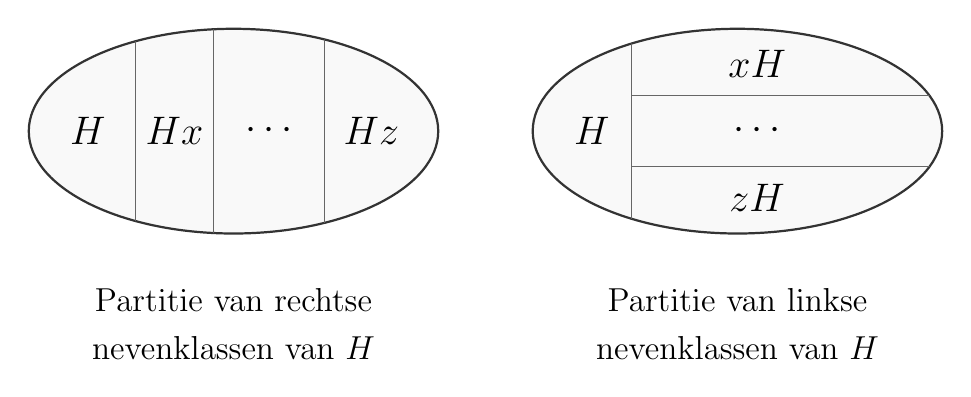
\begin{tikzpicture}[>=latex]

% --- Stijldefinities ---
\tikzset{
    quotientSet/.style={
        fill=gray!5,
        draw=black!80,
        thick
    },
    partitionLine/.style={
        draw=black!60,
        thin
    },
    cosetLabel/.style={
        font=\Large
    },
    captionLabel/.style={
        font=\large,
        align=center
    }
}

% =========================================================
% Linker figuur: Partitie van rechtse nevenklassen
% =========================================================

\draw[quotientSet] (0,0) ellipse (2.6cm and 1.3cm);

% Verticale scheidingslijnen binnen de ellips
\begin{scope}
    \clip (0,0) ellipse (2.6cm and 1.3cm);
    \draw[partitionLine] (-1.25,-1.5) -- (-1.25,1.5);
    \draw[partitionLine] (-0.25,-1.5) -- (-0.25,1.5);
    \draw[partitionLine] (1.15,-1.5) -- (1.15,1.5);
\end{scope}

% Labels
\node[cosetLabel] at (-1.85,0) {$H$};
\node[cosetLabel] at (-0.75,0) {$Hx$};
\node[cosetLabel] at (0.45,0) {$\cdots$};
\node[cosetLabel] at (1.75,0) {$Hz$};

% Onderschrift
\node[captionLabel] at (0,-2.15) {Partitie van rechtse};
\node[captionLabel] at (0,-2.75) {nevenklassen van $H$};


% =========================================================
% Rechter figuur: Partitie van linkse nevenklassen
% =========================================================

\begin{scope}[xshift=6.4cm]

\draw[quotientSet] (0,0) ellipse (2.6cm and 1.3cm);

% Scheidingslijnen binnen de ellips
\begin{scope}
    \clip (0,0) ellipse (2.6cm and 1.3cm);

    % Verticale lijn die H afscheidt
    \draw[partitionLine] (-1.35,-1.5) -- (-1.35,1.5);

    % Horizontale lijnen voor xH, ..., zH
    \draw[partitionLine] (-1.35,0.45) -- (3,0.45);
    \draw[partitionLine] (-1.35,-0.45) -- (3,-0.45);
\end{scope}

% Labels
\node[cosetLabel] at (-1.85,0) {$H$};
\node[cosetLabel] at (0.25,0.85) {$xH$};
\node[cosetLabel] at (0.25,0) {$\cdots$};
\node[cosetLabel] at (0.25,-0.85) {$zH$};

% Onderschrift
\node[captionLabel] at (0,-2.15) {Partitie van linkse};
\node[captionLabel] at (0,-2.75) {nevenklassen van $H$};

\end{scope}

\end{tikzpicture}
}
\end{center}

\begin{nicetheorem}*
    Alle linkernevenklassen (rechternevenklassen) van $H \subseteq G$ staan in bijectie met $H$, en dus ook onderling met elkaar.
    \nextpart[Bewijs.]*
    Neem een $g \in G$ en beschouw de afbeelding:
    \begin{equation*}
        \psi : H \to g*H : h \mapsto g*h
    \end{equation*}
    Deze afbeelding stuurt elke element van $H$ naar een element van de nevenklasse $gH$.
    
    \vspace{0.25cm}

    \underbar{Injectief:} Stel:
    \begin{equation*}
        \begin{aligned}
            \psi(h_1) &= \psi(h_2) \\
            &\Downarrow \\
            g * h_1 &= g * h_2 \\
            &\Downarrow \textcolor{Green}{\text{ $G$ is een groep dus schrappen mag}} \\
            h_1 &= h_2 \\
            &\Downarrow \\
            \text{Dus } &\psi \text{ is injectief}
        \end{aligned}
    \end{equation*}

    \underbar{Surjectief:} Neem een willekeurige $y \in g*H$. Dan bestaat er per definitie een $h \in H$ zodat $y = g * h$. Maar dan:
    \begin{equation*}
        y = \psi(h)
    \end{equation*}
    Dus elk element van $g*H$ wordt bereikt, dus $\psi$ is surjectief. Dus $\psi$ is ook bijectief, en daarom:
    \begin{equation}
        \#(g*H) = \# H \qedtag
    \end{equation}
\end{nicetheorem}

De stelling van Lagrange volgt hier direct uit:

\begin{nicetheorem}*[van Lagrange]
    Zij $\langle G,* \rangle$ een eindige groep en zij $H \subseteq G$ een deelgroep. Dan is
    \begin{equationbox}*[red!75!black]
        \#H\ \mid\ \#G
    \end{equationbox}
    \nextpart[Bewijs.]*
    De linker- of rechternevenklassen van $H$ in $G$ vormen een partitie van $G$. Dwz.
    \begin{enumerate}
        \item elke $g \in G$ zit in een nevenklasse
        \item twee nevenklassen zijn ofwel gelijk ofwel disjunct
        \item alle nevenklassen samen vormen $G$
    \end{enumerate}
    Dus $G$ wordt opgedeeld in stukken:
    \begin{equation*}
        G = g_1*H \cup g_2*H \cup \ldots \cup g_k*H
    \end{equation*}
    waarbij de neveklassen disjunct zijn. Elke nevenklasse heeft evenveel elementen als $H$. Dus:
    \begin{equation*}
        \#G = k \cdot \#H
    \end{equation*}
    Dus 
    \begin{equation*}
        \#H \mid \#G
    \end{equation*}
\end{nicetheorem}

\textbf{\underbar{Terminologie:}} Het aantal linker- of rechternevenklassen $=\frac{\#G}{\#H}$ wordt de \inlinetext{index}[Goldenrod!55] van $H$ in $G$ genoemd. Dit noteer je als $[g:H]$.

\textbf{\underbar{Voorbeeld:}} Beschouw $S_3 = S(\{1,2,3\}) = \{id,\ (1\ 2),\ (1\ 3),\ (2\ 3),\ (1\ 2\ 3),\ (1\ 3\ 2)\}$. Neem een deelgroep $H \subseteq S_3$:
\begin{equation*}
    H = \{id,\ (1\ 2)\}
\end{equation*}
Wat zijn de linkernevenklassen van deze deelgroep $H$?

\underbar{Oplossing:} Omdat $H$ 2 elementen heeft, zal elke linkernevenklasse ook 2 elementen hebben.
\begin{itemize}
    \item $id \circ H = \{id,\ (1\ 2)\} = H$
    \item $(1\ 2) \circ H = \{(1\ 2) \circ id,\ (1\ 2) \circ (1\ 2)\} = \{(1\ 2),\ id\} = H$
\end{itemize}
$\rightarrow$ We hebben hier 2 nevenklassen die hetzelfde zijn, dus je weet al dat:
\begin{equation*}
    id \sim (1\ 2)
\end{equation*}
\begin{itemize}
    \item $(1\ 3) \circ H = \{(1\ 3) \circ id,\ (1\ 3)\circ(1\ 2)\} = \{(1\ 3),\ (1\ 2\ 3)\}$
    \item $(2\ 3) \circ H = \{(2\ 3) \circ id,\ (2\ 3)\circ(1\ 2)\} = \{(2\ 3),\ (1\ 3\ 2)\}$ $\rightarrow$
\end{itemize}
$\rightarrow$ 6 verschillende elementen = alle elementen $S_3$
\begin{equation*}
    S_3 = H \cup (1\ 3)H \cup (2\ 3)H
\end{equation*}




\newpage
\subsection{Orde van een element \& Cyclische groepen}

\textbf{\underbar{Notatie:}} Zij $\langle G,* \rangle$ een groep en zij $g \in G$. Dan is
\begin{equation*}
    \begin{aligned}
        g^n &= \underbrace{g\ *\ g\ *\ \ldots\ *\ g}_{\text{n }g\text{'s}} \qquad n > 0 \\
        g^0 &= e \\
        g^n &= (g^{-1})^{|n|} \qquad \text{als } n<0
    \end{aligned}
\end{equation*}

\begin{nicenote}*[over de notatie $+$]
    \nextpart[]*
    In veel voorbeelden (bv. $\langle \mathbb{Z},+ \rangle$) noteren we de bewerking met $+$.\newline
    $\longrightarrow$ Er zijn 2 conventies in dit geval:
    \begin{itemize}
        \item Deze notatie gebruiken we nooit voor niet-commutatieve gropen.
        \item Voor herhaaldelijke toepassing van $+$ schrijven we $n \cdot g$ ipv. $g^n$.
    \end{itemize}
\end{nicenote}

\begin{nicedefinition}*[Orde]
    \nextpart[]*
    Zij $\langle G,* \rangle$ een groep en zij $g \in G$, dan is de \textcolor{PineGreen!75!black}{\textbf{orde van $g$}} (notatie $\text{ord}(g)$) de kleinste $n \ge 1$ zodat $g^n=e$.

    \vspace{0.15cm}

    $\to$ als dit niet bestaat dan zeggen we: $\text{ord}(g) = \infty$
\end{nicedefinition}

\begin{niceexample}
    Wat is de orde van $(1\ 2\ 3)$ in $S_3$?
\end{niceexample}

\textbf{\underbar{Oplossing:}} We zoeken de kleinste $n \ge 1$ zodat $(1\ 2\ 3)^n = e$:
\begin{itemize}
    \item $(1\ 2\ 3)^1 = (1\ 2\ 3)$
    \item $(1\ 2\ 3)^2 = (1\ 2\ 3) \circ (1\ 2\ 3) = (1\ 3\ 2)$
    \item $(1\ 2\ 3)^3 = (1\ 3\ 2) \circ (1\ 2\ 3) = e$
\end{itemize}
$\to \text{ord}((1\ 2\ 3)) = 3$

\begin{nicedefinition}*[Cyclische groep]
    \nextpart[]*
    Voor een element $g \in G$ noemen we de deelgroep
    \begin{equation*}
        \langle g \rangle = \{g^n \mid n \in \mathbb{Z}\}
    \end{equation*}
    de \textcolor{PineGreen!75!black}{\textbf{cyclische groep voortgebracht door $g$}}. $g$ noemt men een \textcolor{PineGreen!75!black}{\textbf{generator}} en is over het algemeen niet uniek. De notatie $\langle g \rangle$ wilt zeggen "voortgebracht door".

    \vspace{0.25cm}

    Indien dit gans $G$ is noemen we $G$ een \textcolor{PineGreen!75!black}{\textbf{cyclische groep}}.
\end{nicedefinition}

Een \inlinetext{cyclische groep} is een groep die je kan bekomen met één element door dat element herhaaldelijk met zichzelf samen te stellen of door de inverse van dat element herhaaldelijk met zichzelf samen te stellen.

\textbf{\underbar{Voorbeeld:}} De groep $\langle \mathbb{Z},+ \rangle$ is een cyclische groep want ze heeft generator $1$ of $-1$.
\begin{itemize}
    \item $n ge 0$: $1+1+1+ \dots = n \cdot 1$ (dit geeft 1, 2, 3, 4, \dots)
    \item $n=0$: het neutrale element (0)
    \item negatieve $n$: dwz. de inverse van ons element herhaaldelijk optellen. De inverse van $1$ is $-1$. Dus: $(-1) + (-1) + \dots = n \cdot 1$ (dit geeft $-1$, $-2$, \dots)
\end{itemize}
Omdat we met de elementen 1 en zijn inverse -1 alle gehele getallen kunnen bereiken, is $\langle \mathbb{Z},+ \rangle$ een cyclische groep met generator $1$ (of $-1$).

\begin{niceexercise}
    Is de groep $\langle \mathbb{Z}_5 \backslash \{\bar{0}\}, \bullet \rangle$ cyclisch?
\end{niceexercise}

\textbf{\underbar{Oplossing:}} $\mathbb{Z}_5 \backslash \{0\} = \{\bar{1}, \bar{2}, \bar{3}, \bar{4}\}$

Om te kijken of deze groep cyclisch is, moeten we controleren of er minstens één element (een generator) bestaat die in zijn eentje de hele verzameling $\{\bar{1}, \bar{2}, \bar{3}, \bar{4}\}$ kan maken door constant met zichzelf te vermenigvuldigen modulo 5.

\textbf{1. Element 1:}
\begin{itemize}
    \item $1^1 = 1$
    \item $1^2 = 1$\dots Dit blijft altijd $1$. Dit is een cyclische deelgroep $\langle 1 \rangle = \{1\}$. Geen generator voor de hele groep.
\end{itemize}
\textbf{2. Element 2:}
\begin{itemize}
    \item $2^1=2$
    \item $2^2=4$
    \item $2^3=8\equiv3$
    \item $2^4=16\equiv1$
\end{itemize}
Dit geeft $\{2, 4, 3, 1\}$, exact de elementen van de groep. Dus de groep is cyclisch met generator $2$. $3$ is ook generator (analoog).

\begin{nicenote}*
    \nextpart[]*
    Als de orde van $g$ eindig is, dan is
    \begin{equation*}
        \text{ord}(g) = \#\{g^n \mid n \in \mathbb{Z}\}
    \end{equation*}
    want $\{\textcolor{Green}{e}, g, \dots, g^{\text{ord}(g)-1}\}\textcolor{Green}{g^{\text{ord}(g)}}\}$
\end{nicenote}

\begin{nicecorollary}*[van Lagrange 1]\label{gevolg:H3_gevolg_lagrange_1}
    \nextpart[]*
    Je weet: "een element $g$ genereert een deelgroep $\langle g \rangle$. En omdat $\langle g \rangle$ een deelgroep is van $G$, weten we ook uit \emph{Lagrange}:
    \begin{equation*}
        \#\langle g \rangle \mid \#G
    \end{equation*}
    Maar we weten ook dat
    \begin{equation*}
        \#\langle g \rangle = \text{ord}(g)
    \end{equation*}
    Dus: als $G$ eindig is, dan is
    \begin{equation*}
        \text{ord}(g)\mid\#G
    \end{equation*}
\end{nicecorollary}

\begin{nicecorollary}*[van Lagrange 2]\label{gevolg:lagrange_2_gevolg}
    \nextpart[]*
    Als $G$ een eindige groep is, dan geldt voor elke $g \in G$ dat:
    \begin{equation*}
        g^{\#G} = e
    \end{equation*}
\end{nicecorollary}
\textbf{\underbar{Bewijs:}} $\#G = \lambda \cdot \text{ord}(g)$ voor een zekere $\lambda \in \mathbb{Z}$, want $\text{ord}(g)\mid\#G$.

Dus:
\begin{equation*}
    \begin{aligned}
        g^{\#G} &= g^{\lambda \cdot \text{ord}(g)} \\
                &= \left(g^{\text{ord}(g)}\right)^\lambda \\
                &= e^\lambda \\
                &= e
    \end{aligned}
\end{equation*}

\begin{nicecorollary}*[van Lagrange 3]
    \nextpart[]*
    Als $\#G$ een priemgetal is, dan is $G$ cyclisch (en is er op isomorfie na, maar één zo'n groep: $\mathbb{Z}_p$).
\end{nicecorollary}

\textbf{\underbar{Bewijs:}} Stel $\#G = p$ waarbij $p$ een priemgetal is. Neem dan een element $g \in G$ met $g \neq e$. Dan is:
\begin{equation*}
    \text{ord}(g) \neq 1
\end{equation*}
want alleen het neutraal element heeft orde $1$. Uit \emph{Lagrange} weten we nu ook dat:
\begin{equation*}
    \text{ord}(g) \mid \#G = p
\end{equation*}
Maar $p$ is priem. De enige positieve delers van $p$ zijn $1$ en $p$.

Omdat $g \neq e$, kan de orde niet $1$ zijn. Dus:
\begin{equation*}
    \text{ord}(g) = p
\end{equation*}
Dus $\langle g \rangle$ heeft precies $p$ elementen: $\#\langle g \rangle = p$. Maar $G$ heeft ook $p$ elementen. Dus:
\begin{equation*}
    \langle g \rangle = G
\end{equation*}
Daarom is $G$ cyclisch.

\begin{barbox}[Thistle][gray!2]
    \textcolor{Thistle}{\textbf{Teaser:}} \textbf{Kleine stelling van Fermat} $\to$ ingrediënt RSA encryptie

    \vspace{0.25cm}

    Als $p$ een priemgetal is en $a \in \mathbb{Z}$ is niet deelbaar door $p$ ($p \nmid a$), dan:
    \begin{equation*}
        a^{p-1} \equiv 1 \pmod p
    \end{equation*}
    Beschouw de groep $\langle\mathbb{Z}_p\backslash\{\bar{0}\},\cdot\rangle$ (we zullen dit later $\mathbb{Z}_p^{\times}$ noemen). Deze groep heeft $p-1$ elementen. Als $p \nmid a$, dan is $\bar{a} \neq \bar{0}$ (want in $\mathbb{Z}_p$ geldt dat $\bar{a} = \bar{0} \iff a \equiv 0 \pmod{p}$ en dat betekent net $p \mid a$), dus:
    \begin{equation*}
        \bar{a} \in \mathbb{Z}_p^{\times}
    \end{equation*}
    Door \Cref{gevolg:lagrange_2_gevolg} geldt:
    \begin{equation*}
        \bar{a}^{\#\mathbb{Z}_p^{\times}} = \bar{1}
    \end{equation*}
    Omdat $\#\mathbb{Z}_p^{\times} = p-1$ krijg je:
    \begin{equation*}
        \bar{a}^{p-1} = \bar{1}
    \end{equation*}
    Dus:
    \begin{equation*}
        a^{p-1} \equiv 1 \pmod{p}
    \end{equation*}
\end{barbox}

\subsection{Normale deelgroepen en Quotiëntgroepen}

\subsubsection{Inleiding en Motivatie}

We hebben gezien dat een deelgroep $H \subseteq G$ de groep $G$ opdeelt in nevenklassen. De volgende vraag is:
\begin{center}
    Kunnen we met deze nevenklassen zelf rekenen?
\end{center}
Dus kunnen we rekenen met verzamelingen van de vorm:
\begin{equation*}
    gH = \{g*h \mid h \in H\}
\end{equation*}
Als dit kan, krijgen we een nieuwe groep waarvan de elementen de nevenklassen van $H$ in $G$ zijn. Die groep noemen we de quotiëntgroep $G/H$.

\SimpleHeading{Motivatie}

Herinner: als we met de groep $G = \langle \mathbb{Z},+ \rangle$ werken en de deelgroep $H = \langle m\mathbb{Z},+\rangle = \{\dots, -2m,-m,0,m,2m,\dots\}$ voor $m \ge 1$. Dan zijn de nevenklassen:
\begin{equation*}
    a + m\mathbb{Z}
\end{equation*}
Bijvoorbeeld voor $m=5$:
\begin{equation*}
    2 + 5\mathbb{Z} = \{\dots, -8, -3, 2, 7, 12, \dots\}
\end{equation*}
Dit is exact dezelfde equivalentieklasse als:
\begin{equation*}
    \bar{2} \in \mathbb{Z}_5
\end{equation*}
Modulo rekenen is dus eigenlijk rekenen met nevenklassen:
\begin{equation*}
    (a + m\mathbb{Z}) + (b+m\mathbb{Z}) = (a+b) + m\mathbb{Z}
\end{equation*}
Bijvoorbeeld:
\begin{equation*}
    (2 + 5\mathbb{Z}) + (3 + 5\mathbb{Z}) = 5 + 5\mathbb{Z} = 0 + 5\mathbb{Z}
\end{equation*}
Dus
\begin{equation*}
    \bar{2} + \bar{3} = \bar{0} \quad \text{in } \mathbb{Z}_5
\end{equation*}

\SimpleHeading{Link met de equivalentierelatie}

Eerder hadden we bij modulo:
\begin{equation*}
    \begin{aligned}
        a \sim b &\iff m \mid a - b\\
                 &\iff a - b \in m\mathbb{Z}
    \end{aligned}
\end{equation*}
In groepentheorie gebruik je inversen ipv. mintekens. Bij een multiplicatieve groep schrijf je:
\begin{equation*}
    g_1 \sim g_2 \iff g_1^{-1} * g_2 \in H
\end{equation*}
Bij een additieve groep is $g_1^{-1}$ gewoon $-g_1$.
Dus:
\begin{equation*}
    g_1^{-1} * g_2
\end{equation*}
wordt additief:
\begin{equation*}
    -g_1 + g_2 = g_2 - g_1
\end{equation*}
In $\mathbb{Z}$ maakt dat niet uit, want:
\begin{equation*}
    g_2 - g_1 \in m\mathbb{Z} \iff g_1 - g_2 \in m\mathbb{Z}
\end{equation*}

\SimpleHeading{Wat willen we doen voor een algemen groep?}

We hebben een groep $G$ en een deelgroep $H$. De nevenklassen zijn:
\begin{equation*}
    gH
\end{equation*}
We willen de verzameling van nevenklassen een groepsstructuur geven. Dus we definiëren:
\begin{equation*}
    G/H = \{gH \mid g \in G\}
\end{equation*}
En dat wil zeggen:
\begin{equation*}
    (g_1H)(g_2H) = (g_1g_2)H
\end{equation*}
Bijvoorbeeld:
\begin{equation*}
    \text{klasse van }g_1 \cdot \text{ klasse van }g_2 = \text{ klasse van }g_1g_2
\end{equation*}
\emoji{warning}\textbf{Maar dit werkt enkel als het resultaat niet afhangt van de gekozen representanten!}

\SimpleHeading{Het probleem met representanten}

Een nevenklasse $gH$ heeft veel representanten. Als $h_1 \in H$, dan zit ook $g_1h_1$ in dezelfde nevenklasse als $g_1$, want:
\begin{equation*}
    g_1h_1 \in g_1H
\end{equation*}
Dus $g_1$ en $g_1h_1$ stellen dezelfde neveklasse voor.

Indien onze definitie goed is, dan zou moeten gelden:
\begin{equation*}
    (g_1H)(g_2H) = ((g_1h_1)H)((g_2h_2)H)
\end{equation*}
Met andere woorden: als we andere representanten nemen, moeten we dezelfde nevenklasse krijgen. De gewenste uitkomst is:
\begin{equation*}
    (g_1g_2)H
\end{equation*}
Maar met andere representanten krijg je:
\begin{equation*}
    (g_1h_1)(g_2h_2)H
\end{equation*}
Dus:
\begin{equation*}
    g_1*h_1*g_2*h_2*H
\end{equation*}

\underline{$h_2$ kan weg:} Omdat $h_2 \in H$ geldt: $h_2H = H$. Waarom?
\begin{equation*}
    h_2H = \{h_2*h \mid h \in H\}
\end{equation*}
Omdat $H$ een deelgroep is, ligt $h_2*h \in H$, dus 
\begin{equation*}
    h_2 * H \subseteq H
\end{equation*}
Hierdoor geldt dus dat:
\begin{equation*}
    g_1*h_1*g_2*h_2*H = g_1 * h_1 * g_2 * H
\end{equation*}

\underline{Waarom kan $h_1$ niet zomaar weg:} We zitten nu met:
\begin{equation*}
    g_1 * h_1 * g_2 * H
\end{equation*}
We zouden graag willen dat dit gelijk is aan:
\begin{equation*}
    g_1 * g_2 * H
\end{equation*}
Maar $h_1$ staat tussen $g_1$ en $g_2$:
\begin{equation*}
    g_1 * \textcolor{red}{h_1} * g_2 * H 
\end{equation*}
Als de groep commutatief is, dan mag je $h_1$ en $g_2$ verwisselen:
\begin{equation*}
    g_1 * h_1 * g_2 * H = g_1 * g_2 * h_1 * H
\end{equation*}
en dan kan je inderdaad vereenvoudigen want $h_1 * H = H$ want $h_1 \in H$. Dus:
\begin{equation*}
    g_1 * g_2 * h_1 * H = g_1 * g_2 * H
\end{equation*}
\emoji{warning}\textbf{Maar in een niet-commutatieve groep mag dit niet!}

\SimpleHeading{De oplossing: normale deelgroepen}

We hebben een eigenschap nodig die zegt:
\begin{barbox}[PineGreen]
    Je mag elementen van $H$ "langs" elementen van $G$ verschuiven, maar misschien veranderen ze onderweg in een ander element van $H$.
\end{barbox}

Formeel willen we dat voor alle $g \in G$ en $h \in H$:
\begin{equation*}
    g^{-1} * h * g \in H
\end{equation*}
Dit is een van de definities van een \textbf{normale deelgroep}. We noteren dit als:
\begin{equation*}
    H \trianglelefteq G
\end{equation*}
Equivalent hiermee is:
\begin{equation*}
    gH = Hg \qquad \forall g \in G
\end{equation*}
Dus een normale deelgroep is een deelgroep waarvoor de linker- en rechternevenklassen samenvallen.

\SimpleHeading{Hoe lost normaliteit het probleem op?}

We hadden:
\begin{equation*}
    g_1 * h_1 * g_2 * h_2 * H
\end{equation*}
We willen dit herleiden tot:
\begin{equation*}
    g_1 * g_2 * H
\end{equation*}
Het probleemstuk is:
\begin{equation*}
    h_1 * g_2
\end{equation*}
We herschrijven dit als:
\begin{equation*}
    h_1 * g_2 = g_2 * (g_2^{-1} * h_1 * g_2)
\end{equation*}
Check:
\begin{equation*}
    g_2 * (g_2^{-1} * h_1 * g_2) = (g_2 * g_2^{-1}) * h_1 * g_2 = e * h_1 * g_2 = h_1 * g_2
\end{equation*}
Nu komt de normaliteit. Omdat $h_1 \in H$ en $H \trianglelefteq G$, geldt:
\begin{equation*}
    g_2^{-1} * h_1 * g_2 \in H
\end{equation*}
Noem $h' = g_2^{-1} * h_1 * g_2$. Dan is $h' \in H$. En dus:
\begin{equation*}
    h_1 * g_2 = g_2 * h'
\end{equation*}
Dan krijgen we:
\begin{equation*}
    \begin{aligned}
        g_1 * h_1 * g_2 * h_2 * H &= g_1 * g_2 * h' * h_2 * H \\
        &\Downarrow \textcolor{Green}{ h',h_2 \in H \Rightarrow h' * h_2 \in H \Rightarrow h'* h_2 * H = H} \\
        &= g_1 * g_2 * H
    \end{aligned}
\end{equation*}
Conclusie:
\begin{equation*}
    (g_1 * H) * (g_2 * H) = (g_1 * g_2) * H
\end{equation*}
is goed gedefinieerd als $H$ normaal is.

\SimpleHeading{Waarom is dit goed gedefinieerd?}

Goed gedefinieerd betekent hier:
\begin{barbox}[PineGreen]
    Het resultaat hangt niet af van de gekozen representanten.
\end{barbox}
Dus als:
\begin{equation*}
    g_1 * H = g_1' * H
\end{equation*}
en
\begin{equation*}
    g_2 * H = g_2' * H
\end{equation*}
dan moet gelden:
\begin{equation*}
    (g_1 * g_2) * H = (g_1' * g_2') * H
\end{equation*}
Bij normale deelgroepen is dat waar. Daarom kan je van de neveklassen zelf een groep maken!

\SimpleHeading{De quotiëntgroep}

Als $\H \trianglelefteq G$, dan definiëren we:
\begin{equation*}
    G/H = \{gH \mid g \in G\}
\end{equation*}
De bewerking is:
\begin{equation*}
    (g_1H)(g_2H) = (g_1g_2)H
\end{equation*}
Dan is $G/H$ een groep. Het neutraal element is:
\begin{equation*}
    H = eH
\end{equation*}
De inverse van $gH$ is:
\begin{equation*}
    g^{-1}H
\end{equation*}
Want:
\begin{equation*}
    (gH)(g^{-1}H) = (gg^{-1})H = eH = H
\end{equation*}

\SimpleHeading{Terug naar voorbeeld $\mathbb{Z}/m\mathbb{Z}$}

Waarom werkt dit altijd bij $\mathbb{Z}/m\mathbb{Z}$? $\to$ omdat $\mathbb{Z}$ abels is! In een abelse groep is elke deelgroep normaal. Dus:
\begin{equation*}
    m\mathbb{Z} \trianglelefteq \mathbb{Z}
\end{equation*}
Daarom mag je de quotiëntgroep maken:
\begin{equation*}
    \mathbb{Z}/m\mathbb{Z}
\end{equation*}
De elementen zijn:
\begin{equation*}
    0 + m\mathbb{Z},\ 1 + m\mathbb{Z},\dots,\ (m-1) + m\mathbb{Z}
\end{equation*}
En de bewerking is:
\begin{equation*}
    (a + m\mathbb{Z}) + (b + m\mathbb{Z}) = (a + b) + m\mathbb{Z}
\end{equation*}
Dat is precies rekenen modulo $m$!

\newpage
\subsubsection{Normaaldeler}

\begin{nicedefinition}*[Toegevoegde elementen en conjugatie]
    \nextpart[]*
    Voor $x,g \in G$ heet $g^{-1}xg$ het \textcolor{PineGreen!75!black}{\textbf{toegevoegde (geconjugeerde) element}} van $x$ onder $g$.
\end{nicedefinition}

\textbf{\underbar{Intuïtief:}} Conjugeren betekent "$x$ bekijken vanuit het standpunt van $g$". Het is een soort coördinatenwissel. In een abelse groep verandert er niets want:
\begin{equation*}
    g^{-1}xg = g^{-1}gx = x
\end{equation*}

\begin{nicetheorem}*
    \nextpart[]*
    Voor $x,y,g \in G$:
    \begin{enumerate}
        \item Als $gx = xg$, dan geldt: $g^{-1}xg=x$ (dit geldt dus altijd in een abelse groep).
        \item Is $y$ de toegevoegde van $x$ door $g$, dan is $x$ de toegevoegde van $y$ door $g^{-1}$.
        \begin{equation*}
            \begin{aligned}
                y &= g^{-1}xg \\
                &\Downarrow \textcolor{Green}{\text{ Links $g$ en rechts $g^{-1}$}}\\
                gyg^{-1} &= x
            \end{aligned}
        \end{equation*}
        \item Voor een vaste $g$ is $\psi : G \to G : x \mapsto g^{-1}xg$ een automorfisme. Want:
        \begin{equation*}
            \psi(xy) = g^{-1}xyg = g^{-1}x\textcolor{Green}{gg^{-1}}yg = \psi(x)\psi(y)
        \end{equation*}
    \end{enumerate}
\end{nicetheorem}

\begin{nicedefinition}*[Normaaldeler]
    \nextpart[]*
    Een deelgroep $H$ is een \textcolor{PineGreen!75!black}{\textbf{normaaldeler}} van $G$ als ze invariant is onder \textbf{alle} innerlijke automorfismen:
    \begin{equation*}
        g^{-1}Hg = H \quad \forall g \in G. \qquad \text{Notatie: } H \trianglelefteq G 
    \end{equation*}
\end{nicedefinition}

\textbf{\underbar{Twee gratis gevallen:}}
\begin{itemize}
    \item In een abelse groep is elke deelgroep een normaaldeler.
    \item Een deelgroep van \textbf{index 2} is altijd een normaaldeler. Want er is maar één nevenklasse buiten $H$, en die is noodzakelijk zowel links als rechts.
\end{itemize}

\begin{nicetheorem}*[Bruikbare criterium]
    \nextpart[]*
    $H$ is een normaaldeler $\iff$ alle linkse nevenklassen zijn ook rechtse nevenklassen.
    \begin{equation*}
        gH = Hg \qquad \forall g \in G
    \end{equation*}
    Dit is meestal de gemakkelijkste manier om normaliteit na te gaan.
\end{nicetheorem}

\begin{nicetheorem}*[Wanneer is $\circledast$ goed gedefinieerd?]
    \nextpart[]*
    \begin{equation*}
        \begin{aligned}
            xH \circledast yH &= (xH)(yH) \text{ is goed gedefinieerd} \\
            &\Updownarrow \\
            H \text{ is een}&\text{ normaaldeler}
        \end{aligned}
    \end{equation*}
    En dan geldt de simpele formule:
    \begin{equation*}
        (xH)(yH) = xyH
    \end{equation*}
    Want:
    \begin{equation*}
        (xH)(yH) = x(Hy)H = x(yH)H = xy(HH) = xyH
    \end{equation*}
\end{nicetheorem}

\subsubsection{Quotiëntgroep}

\begin{nicedefinition}*[Quotiëntgroep]
    \nextpart[]*
    Is $H \trianglelefteq G$, dan is $\langle G/H,\ \circledast \rangle$ een groep, namelijk de \textcolor{PineGreen!75!black}{\textbf{quotiëntgroep}} $G/H$. Het neutraal element is $H$ zelf ($=eH$); de inverse van $xH = x^{-1}$.
\end{nicedefinition}

\textbf{\underbar{Intuïtief:}} De quotiëntgroep ontstaat door heel $H$ "plat te drukken" tot één punt (het nieuwe neutrale element). Alles wat in $H$ zat, telt nu als "gelijk aan $e$". De andere nevenklassen worden de overige elementen. Dit is precies wat $\mathbb{Z}/n\mathbb{Z} = \mathbb{Z}_n$ doet: alle veelvouden van $n$ worden "gelijk aan 0", en je houdt $\{\bar{0},\ \bar{1},\ \ldots,\ \overline{n-1}\}$ over. Modulo rekenen is dus gewoon een quotiëntgroep. 

\subsubsection{Homomorfismen tussen groepen}

\begin{nicedefinition}*[Groep-homomorfisme en Kern]
    \nextpart[]*
    Een \textcolor{PineGreen!75!black}{\textbf{groep-homomorfisme}} $\psi:G\to H$ bewaart de bewerking
    \begin{equation*}
        \psi(xy) = \psi(x)\psi(y)
    \end{equation*}
    De \textcolor{PineGreen!75!black}{\textbf{kern}} is
    \begin{equation*}
        \text{ker }\psi = \{g \in G \mid \psi(g) = e_H\}
    \end{equation*}
    Dwz. alles wat naar het neutraal element wordt gestuurd.
\end{nicedefinition}

\textbf{\underbar{Intuïtief:}} De kern is "wat platgedrukt wordt". Een homomorfisme is een soort projectie: ze gooit informatie weg. De kern meet \emph{hoeveel} informatie. Hoe groter de kern, hoe meer er versmolten wordt.

\newpage
\begin{nicetheorem}*[Twee fundamentele feiten]
    \nextpart[]*
    \begin{enumerate}
        \item $\text{ker }\psi$ is altijd een normaaldeler van $G$.
        \item $\psi$ is injectief $\iff$ $\text{ker }\psi = \{e_G\}$
    \end{enumerate}
\end{nicetheorem}

\textbf{\underbar{Merk op:}} $\text{ker }\psi$ is een deelgroep (want gesloten onder product en inverse, beiden gaan naar $e_H$). Ze is ook normaal want voor:
\begin{equation*}
    a \in \operatorname{ker}\psi \qquad \text{en} \qquad g \in G
\end{equation*}
is:
\begin{equation*}
    \psi(g^{-1}ag) = \psi(g)^{-1}\ e_H\ \psi(g) = e_H
\end{equation*}
dus:
\begin{equation*}
    g^{-1}ag \in \operatorname{ker}\psi
\end{equation*}

\textbf{\underbar{Intuïtief:}} Een homomorfisme is injectief precies als het niets "samenplakt", en het enige wat sowieso al naar $e_H$ gaat is $e_G$. Zit er nog iets anders in de kern, dan worden er minstens twee dingen versmolten.

\begin{nicetheorem}*[Het beeld is een deelgroep]
    \nextpart[]*
    $\operatorname{Ran} \psi = \psi(G)$ is een deelgroep van $H$
\end{nicetheorem}

\begin{nicetheorem}*[eerste isomorfiestelling]
    \nextpart[]*
    Zij $\psi: G \to H$ een groeps-homomorfisme met $K = \operatorname{ker}\psi$. Dan:
    \begin{equation*}
        G/K \cong \operatorname{Ran}\psi
    \end{equation*}
    via het isomorfisme
    \begin{equation*}
        \psi: Kg \mapsto \psi(g)
    \end{equation*}
\end{nicetheorem}

\textbf{\underbar{Merk op:}} Deze stelling vat dit hele deel samen. Als je een groep door de kern van een homomorfisme "platgedrukt", dan krijg je exact het beeld terug. We hebben dit eerder al eens gezien als de \textbf{ontbindingsstelling} (\Cref{stelling:H3_ontbindingsstelling}). Het homomorfisme ontbindt canoniek als:
\begin{equation*}
    \psi = i \circ \varphi \circ \pi
\end{equation*}
met:
\begin{itemize}
    \item $\pi : G \to G/K$ de projectie,
    \item $\varphi$ het isomorfisme,
    \item en $i$ de inlassing van $\operatorname{Ran}\psi$ in $H$
\end{itemize}

\begin{center}
\resizebox{0.99\textwidth}{!}{%
    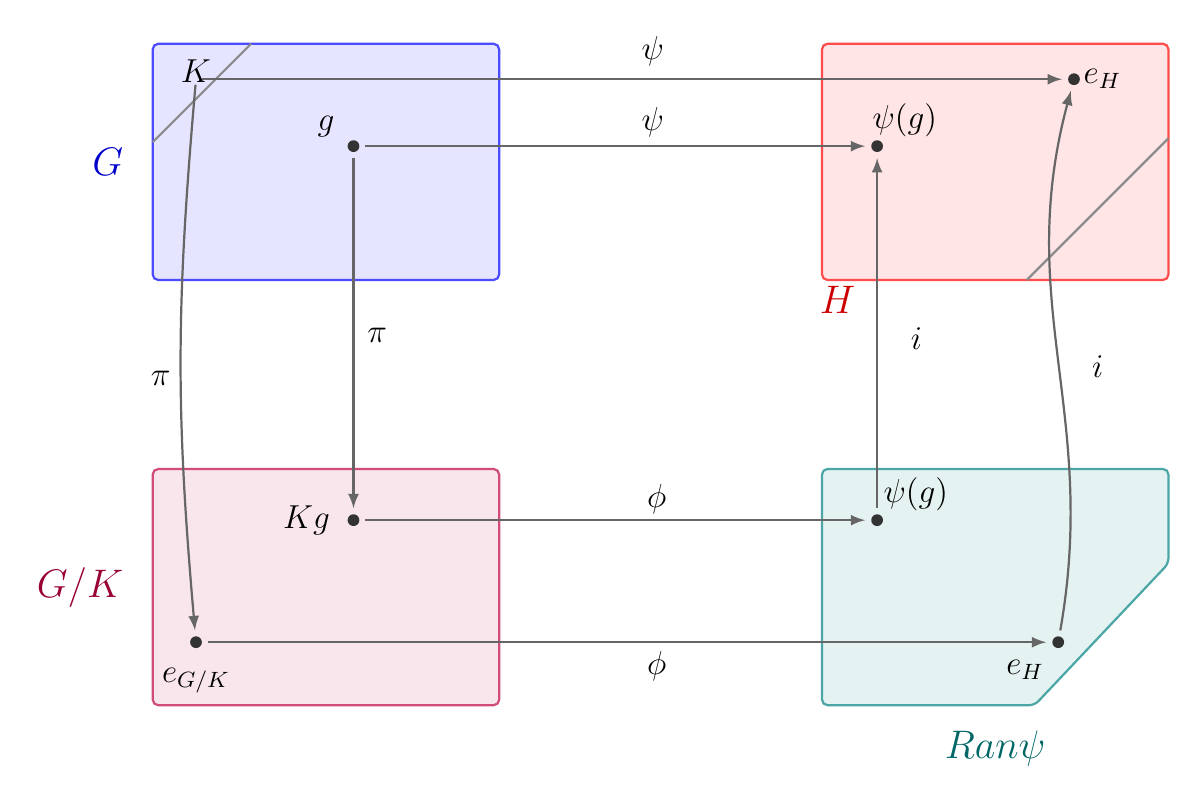
\begin{tikzpicture}[>=latex]

% --- Global TikZ Styles ---
\tikzset{
    setA/.style={fill=blue!10, draw=blue!70, thick, rounded corners=2pt},
    setB/.style={fill=red!10, draw=red!70, thick, rounded corners=2pt},
    setC/.style={fill=purple!10, draw=purple!70, thick, rounded corners=2pt},
    setD/.style={fill=teal!10, draw=teal!70, thick, rounded corners=2pt},
    labelA/.style={text=blue!80!black, font=\Large\bfseries},
    labelB/.style={text=red!80!black, font=\Large\bfseries},
    labelC/.style={text=purple!80!black, font=\Large\bfseries},
    labelD/.style={text=teal!80!black, font=\Large\bfseries},
    point/.style={circle, fill=black!80, inner sep=1.5pt},
    arrow/.style={
        ->,
        >=latex,
        thick,
        draw=black!60,
        shorten >=2pt,
        shorten <=2pt
    },
    innerline/.style={draw=black!45, thick},
    element/.style={font=\large}
}

% ==================================================
% --- Vier verzamelingen / objecten ---
% ==================================================

% --- G linksboven ---
\path[setA] (-2.2, 2.8) rectangle (2.2, 5.8);
\node[labelA, anchor=east] at (-2.45, 4.3) {$G$};
\node[element] at (-1.65, 5.45) {$K$};

% Diagonale lijn in G, zoals in het origineel
\draw[innerline] (-2.2, 4.55) -- (-0.95, 5.8);

% --- H rechtsboven ---
\path[setB] (6.3, 2.8) rectangle (10.7, 5.8);
\node[labelB, anchor=west] at (6.15, 2.55) {$H$};

% Diagonale lijn in H
\draw[innerline] (8.9, 2.8) -- (10.7, 4.6);

% --- G/K linksonder ---
\path[setC] (-2.2, -2.6) rectangle (2.2, 0.4);
\node[labelC, anchor=east] at (-2.45, -1.1) {$G/K$};

% --- Ran psi rechtsonder, met afgesneden hoek ---
\path[setD]
    (6.3, -2.6) --
    (9.0, -2.6) --
    (10.7, -0.8) --
    (10.7, 0.4) --
    (6.3, 0.4) --
    cycle;

\node[labelD] at (8.5, -3.15) {$\operatorname{Ran}\psi$};

% ==================================================
% --- Punten ---
% ==================================================

% Punten in G
\coordinate (K) at (-1.65, 5.35);

\node[point] (g) at (0.35, 4.50) {};
\node[element] at (0.00, 4.75) {$g$};

% Punten in H
\node[point] (psigH) at (7.00, 4.50) {};
\node[element, anchor=south, xshift=10pt] at (psigH) {$\psi(g)$};

\node[point] (eHH) at (9.5, 5.35) {};
\node[element, anchor=west] at (9.5, 5.35) {$e_H$};

% Punten in G/K
\node[point] (Kg) at (0.35, -0.25) {};
\node[element, anchor=east, xshift=-5pt] at (Kg) {$Kg$};

\node[point] (eGK) at (-1.65, -1.80) {};
\node[element, anchor=north] at (-1.65, -2.0) {$e_{G/K}$};

% Punten in Ran psi
\node[point] (psigR) at (7.00, -0.25) {};
\node[element, anchor=south, xshift=14pt] at (psigR) {$\psi(g)$};

\node[point] (eHR) at (9.30, -1.80) {};
\node[element, anchor=north, xshift=-12pt, yshift=-3pt] at (eHR) {$e_H$};

% ==================================================
% --- Pijlen ---
% ==================================================

% psi: G -> H
\draw[arrow] (K) -- (eHH);
\node[element] at (4.15, 5.70) {$\psi$};

\draw[arrow] (g) -- (psigH);
\node[element] at (4.15, 4.8) {$\psi$};

% pi: G -> G/K
\draw[arrow] (K) to[out=-95, in=95, looseness=1.05] (eGK);
\node[element] at (-2.1, 1.55) {$\pi$};

\draw[arrow] (g) -- (Kg);
\node[element] at (0.65, 2.10) {$\pi$};

% phi: G/K -> Ran psi
\draw[arrow] (Kg) -- (psigR);
\node[element] at (4.20, 0.02) {$\phi$};

\draw[arrow] (eGK) -- (eHR);
\node[element] at (4.20, -2.10) {$\phi$};

% i: Ran psi -> H
\draw[arrow] (psigR) -- (psigH);
\node[element] at (7.5, 2.05) {$i$};

\draw[arrow] (eHR) to[out=80, in=-105, looseness=1.05] (eHH);
\node[element] at (9.80, 1.70) {$i$};

\end{tikzpicture}
}
\end{center}

\textbf{\underbar{Voorbeeld:}} 

\begin{description}
    \item[Gegeven:] De afbeelding $f: \mathbb{Z} \to \mathbb{Z}_m : n \mapsto \bar{n}$, waarbij $f$ een groeps-homomorfisme is.
    \item[Gevraagd:] \
    \begin{enumerate}
        \item Bepaal de kern ($\ker f$) van deze afbeelding.
        \item Pas de eerste isomorfiestelling toe om de structurele relatie tussen $\mathbb{Z}$ en $\mathbb{Z}_m$ aan te tonen.
    \end{enumerate}
    \item[Oplossing:] \
    \begin{enumerate}
        \item \textbf{Kern bepalen:} De kern bestaat uit alle elementen die op het neutrale element ($\bar{0}$) worden afgebeeld. Dit zijn precies de veelvouden van $m$:
        $$ \ker f = m\mathbb{Z} $$
        \item \textbf{Isomorfiestelling toepassen:} Omdat $f$ een groeps-homomorfisme is, geeft de eerste isomorfiestelling ($\mathbb{Z}/\ker f \cong f(n)$) meteen het structurele resultaat:
        $$ \mathbb{Z}/m\mathbb{Z} \;\cong\; \mathbb{Z}_m $$
    \end{enumerate}
\end{description}

\newpage
\textbf{\underbar{Voorbeeld:}} 
\begin{description}
    \item[Gegeven:] Een cyclische groep $\langle G, \cdot \rangle$ van orde $n$ met generator $g$, en de afbeelding:
    $$ \psi: \langle\mathbb{Z}, +\rangle \to \langle G, \cdot\rangle : k \mapsto g^k $$
    waarbij $\psi$ een surjectief groepshomomorfisme is.
    
    \item[Gevraagd:] \
    \begin{enumerate}
        \item Bepaal de kern ($\ker\psi$) van deze afbeelding.
        \item Pas de eerste isomorfiestelling toe om te bewijzen dat elke cyclische groep van orde $n$ isomorf is met $\mathbb{Z}_n$.
    \end{enumerate}
    
    \item[Oplossing:] \
    \begin{enumerate}
        \item \textbf{Kern bepalen:} De kern bestaat uit alle elementen $k \in \mathbb{Z}$ die op het neutrale element $e \in G$ worden afgebeeld. Omdat $G$ orde $n$ heeft, geldt $g^k = e$. Wanneer is $g^k=e$? $g^{0}=e$, $g^n=e$, $g^{2n}=e$, $g^{3n}=e$, $g^{-n}=e$, \dots. Kortom, $g^k=e$ als $k$ een veelvoud is van $n$, dus als $n$ een deler is van $k$ ($n \mid k$). Dit zijn precies de veelvouden van $n$:
        $$ \ker\psi = n\mathbb{Z} $$
        
        \item \textbf{Isomorfiestelling toepassen:} Aangezien $\psi$ een surjectief homomorfisme is, is het beeld $\psi(\mathbb{Z}) = G$. De eerste isomorfiestelling ($\mathbb{Z}/\ker\psi \cong \psi(\mathbb{Z})$) geeft dan direct het gezochte structurele resultaat:
        $$ \mathbb{Z}/n\mathbb{Z} = \mathbb{Z}_n \;\cong\; G $$
    \end{enumerate}
\end{description}

\begin{nicecorollary}*[Gevolg van vorig voorbeeld]
    \nextpart[]*
    \textbf{Elke} cyclische groep van orde $n$ is isomorf met $\mathbb{Z}_n$. Er bestaat dus op isomorfie na, maar \textbf{één} cyclische groep per orde!
\end{nicecorollary}

\subsection{Rode draad van dit hoofdstuk}

\begin{roundbox}[CornflowerBlue!10][RoyalPurple]
    Een deelgroep $H$ verdeelt $G$ in \textbf{even grote nevenklassen} ($\Rightarrow$ Lagrange: $\#H \mid \#G)$. Wil je van die nevenklassen een nieuwe groep maken, dan moet $H$ een \textbf{normaaldeler} zijn ($gH=Hg$); dan bestaat de \textbf{quotiëntgroep} $G/H$, die $H$ platdrukt tot het neutraal element. Elk \textbf{homomorfisme} $\psi$ levert automatisch zo'n normaaldeler (de \textbf{kern}), en de \textbf{isomorfiestelling} zegt $G/\operatorname{kern}\psi \cong \operatorname{Ran}\psi$: platdrukken via de kern reconstrueert precies het beeld. Omgekeerd bouw je grotere groepen op via \textbf{direct product}.
\end{roundbox}
\subsection{Oefeningen}





